\documentclass[11pt]{article}
\usepackage{../cs70,latexsym,epsf}
\lecture{16}
\def\title{Note \the\lecturenumber}

%%% Alistair's Macros
\makeatletter
\def\eqalign#1{\,\vcenter{\openup\jot\m@th
  \ialign{\strut\hfil${##}$&${{}##}$\hfil
      \crcr#1\crcr}}\,}
\def\eqalignno#1{\displ@y \tabskip\@centering
  \halign to\displaywidth{\hfil${##}$\tabskip\z@skip
    &${{}##}$\hfil\tabskip\@centering
    &\llap{$##$}\tabskip\z@skip\crcr
    #1\crcr}}
\makeatother
\def\third{{\textstyle{1\over 3}}}
\def\half{{\textstyle{1\over 2}}}
\def\quarter{{\textstyle{1\over 4}}}
\def\ul#1{\underline{#1}}
\def\VarOmega{\mathchar"10A }
\def\varOmega{\mathchar"10A }
\newenvironment{proposition}{\par\global\advance\theoremnumber by 1
{\bf Proposition \the\lecturenumber.\the\theoremnumber}:
\begingroup\em}%
{\endgroup}
\def\ignore#1{}
\def\Ex#1{{\rm E}(#1)}
\def\Var#1{{\rm Var}(#1)}
\def\Aset{{\cal A}}
%%% End Alistair's Macros


\newcounter{thm}
\addtocounter{thm}{\the\lecturenumber}
\newtheorem{lemma}{Lemma}[thm]
\newtheorem{corollary}{Corollary}[thm]
\newtheorem{theorem}{Theorem}[thm]
\newtheorem{definition}{Definition}[thm]



\begin{document}
\maketitle

\section*{A Brief Introduction to Continuous Probability}
Up to now we have focused exclusively on {\it discrete\/} probability spaces~$\Omega$,
where the number of sample points $\omega\in\Omega$ is either finite or countably
infinite (such as the integers).  As a consequence, we have only been able to talk about
{\it discrete\/} random variables, which take on only a finite or countably infinite number
of values.

But in real life many quantities that we wish to model probabilistically are {\it real-valued\/};
examples include the position of a particle in a box, the time at which an certain incident happens,
or the direction of travel of a meteorite.  In this lecture, we discuss how to extend the concepts
we've seen in the discrete setting to this {\em continuous} setting.  As we shall see, everything
translates in a natural way once we have set up the right framework.  The framework involves
some elementary calculus but (at this level of discussion) nothing too scary.


\subsection*{Continuous Uniform Probability Space}

Suppose we spin a ``wheel of fortune" and record the position of the pointer on
the outer circumference of the wheel.  Assuming that the circumference is of length~$\ell$
and that the wheel is unbiased, the position is presumably equally likely to take on
any value in the real interval $[0,\ell]$.  How do we model this experiment using a
probability space?

Consider for a moment the analogous discrete setting, where the pointer
can stop only at a finite number~$m$ of positions distributed evenly around the
wheel. (If $m$ is very large, then this is in some sense similar to the
continuous setting, which we can think of as the limit $m \to \infty$.)
Then we would model this situation using the discrete sample space
$\Omega = \{0,\frac{\ell}{m},\frac{2\ell}{m},\ldots,\frac{(m-1)\ell}{m}\}$, with
uniform probabilities $\Pr[\omega] = \frac{1}{m}$ for each $\omega\in\Omega$.

In the continuous setting, however, we get into trouble if we try the same approach.
If we let $\omega$ range over all real numbers in $\Omega = [0,\ell]$, what value should
we assign to each $\Pr[\omega]$?  By uniformity, this probability should be the
same for all~$\omega$. But if we assign $\Pr[\omega]$ to be any positive value, then
because there are infinitely many $\omega$ in $\Omega$,  the sum
of all probabilities $\Pr[\omega]$ will be~$\infty$! Thus, $\Pr[\omega]$ must be zero for all $\omega\in\Omega$.
But if all of our sample points have probability zero, then we are unable to assign meaningful probabilities
to any events!

To resolve this problem, consider instead any non-empty {\it interval\/} $[a,b]\subseteq[0,\ell]$.
Can we assign a non-zero probability value to this interval?  Since the total probability
assigned to $[0,\ell]$ must be~1, and since we want our probability to be uniform, the
logical value for the probability of interval $[a,b]$ is $$
   \frac{\hbox{\rm length of $[a,b]$}}{\hbox{\rm length of $[0,\ell]$}} = \frac{b-a}{\ell}.  $$
In other words, the probability of  an interval is proportional to its length.

Note that intervals are subsets of the sample space $\Omega$ and are
therefore {\em events}. So in contrast to discrete probability, where we assigned
probabilities to {\em points} in the sample space, in continuous probability we are
assigning probabilities to certain basic events (in this case intervals). What about probabilities of other events?
By specifying the probability of intervals, we have also
specified the probability of any event $E$ which can be written as
the disjoint union of (a finite or countably infinite number of)
intervals, $E=\cup_i E_i$. For then we can write $\Pr[E] = \sum_i
\Pr[E_i]$, in analogous fashion to the discrete case.  Thus for
example the probability that the pointer ends up in the first or
third quadrants of the wheel is
$\frac{\ell/4}{\ell}+\frac{\ell/4}{\ell} = \frac{1}{2}$. For all
practical purposes, such events are all we really need.\footnote{A
formal treatment of which events can be assigned a well-defined
probability requires a discussion of {\it measure theory}, which is
beyond the scope of this course.}


\section*{Continuous Random Variables}
Recall that in the discrete setting we typically work with {\it random variables\/} and
their distributions, rather than directly with probability spaces and events.  The simplest
example of a continuous random variable is the position~$X$ of the pointer in the
wheel of fortune, as discussed above.  This random variable has the {\it uniform\/}
distribution on $[0,\ell]$.  How, precisely, should we define the distribution of a
continuous random variable?  In the discrete case the distribution of a r.v.~$X$
is described by specifying, for each possible value~$a$, the probability $\Pr[X=a]$.
But for the r.v.~$X$ corresponding to the position of the pointer, we have $\Pr[X=a]=0$
for every~$a$, so we run into the same problem as we encountered above in defining
the probability space.

The resolution is the same: instead of specifying $\Pr[X=a]$, we
specify $\Pr[a\le X\le b]$ for  all intervals $[a,b]$.\footnote{Note that it does not matter
whether or not we include the endpoints $a,b$; since $\Pr[X=a]=\Pr[X=b]=0$, we
have $\Pr[a< X< b] = \Pr[a\le X\le b]$.}  To do this formally, we need to introduce
the concept of a {\it probability density function\/} (sometimes  referred to just as
a ``density", or a ``pdf").
\begin{definition}[Density]
A {\em probability density function} for a real-valued random variable~$X$ is a function
$f:\R\to\R$ satisfying:
\begin{enumerate}
  \item $f$ is non-negative: $f(x) \ge 0$ for all $x \in \R$.
  \item The total integral of $f$ is equal to $1$: $\int_\infty^\infty f(x) \, dx = 1$.
\end{enumerate}
Then the distribution of $X$ is given by:
 $$\Pr[a\le X\le b] = \int_{a}^b f(x) dx\qquad\hbox{\rm for all $a\le b$}.  $$
\end{definition}

Let's examine this definition.   Note that  the definite integral is  just the area
under the curve~$f$ between the values~$a$ and~$b$.  Thus $f$ plays a similar
role to the ``histogram" we sometimes draw to picture the distribution of a
discrete random variable.  The first condition that $f$ be non-negative ensures
that the probability of every event is non-negative. The second condition that the
total integral of $f$ equal to $1$ ensures that it defines a valid probability distribution,
because the r.v.~$X$ must take on real values:
\begin{equation}\label{eq:total}
 \Pr[X \in \R] = \Pr[-\infty < X < \infty] = \int_{-\infty}^\infty f(x) dx =  1.
\end{equation}



For example, consider the wheel-of-fortune r.v.~$X$, which has uniform distribution
on the interval $[0,\ell]$. This means the density $f$ of $X$ vanishes outside this interval:
$f(x)=0$ for $x<0$ and for $x>\ell$.  Within the interval $[0,\ell]$ we want
the distribution of~$X$ to be uniform, which means we should take $f$ to be a constant $f(x)=c$
for $0\le x\le\ell$. The value of~$c$ is determined by
the requirement~(\ref{eq:total}) that the total area under $f$ is~1:
$$1 = \int_{-\infty}^\infty f(x) dx = \int_{0}^\ell c \, dx = c\ell,$$
which gives us $c=\frac{1}{\ell}$. Therefore, the density of the uniform
distribution on $[0,\ell]$ is given by $$
   f(x) = \begin{cases}
       0 & \hbox{\rm for $x<0$;}\cr
       1/\ell & \hbox{\rm for $0\le x\le\ell$;}\cr
       0 & \hbox{\rm for $x>\ell$.}\cr
   \end{cases}  $$

\paragraph{Remark:} Following the ``histogram" analogy above,
it is tempting to think of~$f(x)$ as a ``probability."  However,
$f(x)$ doesn't itself correspond to the probability of anything! In particular,
\ul{there is no requirement that} \ul{$f(x)$ be bounded by~1}. For example,
the density of the uniform distribution on the interval $[0,\ell]$ with $\ell = \frac{1}{2}$ is equal to
$f(x) = 1/(\frac{1}{2}) = 2$ for $0 \le x \le \frac{1}{2}$, which is greater than $1$.
To connect density $f(x)$ with probabilities,
we need to look at a very small interval $[x,x+\delta]$ close
to~$x$; then we have
\begin{equation}
\label{eq:small}
   \Pr[x\le X\le x+\delta] = \int_{x}^{x+\delta} f(z) dz \approx \delta f(x).
\end{equation}
Thus, we can interpret $f(x)$ as the ``probability per unit length" in the vicinity
of~$x$.


\subsection*{Expectation and Variance}

As in the discrete case, we define the expectation of a
continuous r.v.\ as follows:
\begin{definition}[Expectation]
The expectation of a continuous r.v.~$X$ with probability
density function~$f$ is $$
   \Ex{X} = \int_{-\infty}^\infty xf(x) dx.  $$
\end{definition}

Note that the integral plays the role of the summation in the
discrete formula $\Ex{X} = \sum_a a\Pr[X=a]$. Similarly, we can define
the variance as follows:

\begin{definition}[Variance]
The variance of a continuous r.v.~$X$ with probability
density function~$f$ is $$
   \Var{X} = \Ex{(X-\Ex{X})^2} = \Ex{X^2} - \Ex{X}^2 = \int_{-\infty}^\infty x^2 f(x) dx \;- \left(\int_{-\infty}^\infty xf(x) dx\right)^2.  $$
\end{definition}


{\bf Example:} Let $X$ be a uniform r.v.\ on the interval
$[0,\ell]$. Then intuitively, its expected value should be in the middle, $\frac{\ell}{2}$.
Indeed, we can use our definition above to compute
$$ \Ex{X} = \int_{0}^\ell x\frac{1}{\ell} dx = \left[\frac{x^2}{2\ell}\right]_0^\ell = \frac{\ell}{2}, $$
as claimed. We can also calculate its variance using the above definition
and plugging in the value $\Ex{X} = \frac{\ell}{2}$ to get:
$$ \Var{X} = \int_{0}^\ell x^2\frac{1}{\ell}dx - \Ex{X}^2 = \left[\frac{x^3}{3\ell}\right]_0^\ell - \left(\frac{\ell}{2}\right)^2 = \frac{\ell^2}{3} - \frac{\ell^2}{4} = \frac{\ell^2}{12}.  $$
The factor of $\frac{1}{12}$ here is not particularly intuitive, but
the fact that the variance is proportional to~$\ell^2$ should come
as no surprise. Like its discrete counterpart, this distribution has
large variance.


\subsection*{Joint Distribution}

Recall that for discrete random variables $X$ and $Y$, their joint
distribution is specified by the probabilities $\Pr[X = a, Y = c]$ for 
all possible values $a,c$. Similarly, if $X$ and $Y$ are continuous
random variables, then their joint distributions are specified by
the probabilities $\Pr[a \le X \le b, c \le Y \le d]$ for all $a \le b$, $c \le d$.
Moreover, just as the distribution of $X$ can be characterized
by its density function, the joint distribution of $X$ and $Y$ can be
characterized by their joint density.

\begin{definition}[Joint Density]
A {\em joint density function} for two random variable~$X$ and $Y$
is a function $f:\R^2\to\R$ satisfying:
\begin{enumerate}
  \item $f$ is non-negative: $f(x,y) \ge 0$ for all $x,y \in \R$.
  \item The total integral of $f$ is equal to $1$: $\int_{-\infty}^\infty \int_{-\infty}^\infty f(x,y) \, dx \, dy = 1$.
\end{enumerate}
Then the joint distribution of $X$ and $Y$ is given by:
 $$ \Pr[a\le X\le b, ~ c \le Y \le d] = \int_{c}^d \int_a^b f(x,y) \, dx \, dy\qquad\hbox{\rm for all $a\le b$ and $c \le d$}.  $$
\end{definition}


In analogy with
(\ref{eq:small}), we can connect the joint density $f(x,y)$ with probabilities by
looking at a very small square $[x,x+\delta] \times [y,y+\delta]$
close to~$(x,y)$; then we have
\begin{equation}
\label{eq:small_joint}
   \Pr[x\le X\le x+\delta, ~ y \le Y \le y +\delta]
= \int_y^{y+\delta}\int_{x}^{x+\delta} f(u,v) \, du \, dv \approx \delta^2
f(x,y).
\end{equation}
Thus we can interpret $f(x,y)$ as the ``probability per unit area"
in the vicinity of~$(x,y)$.

\subsection*{Independence}

Recall that two discrete random variables $X$ and $Y$ are said
to be independent if the events $X=a$ and $Y=c$ are
independent for every possible values $a,c$. We have a similar definition
for continuous random variables:

\begin{definition}[Independence for Continuous R.V.'s]
Two continuous r.v.'s $X,Y$ are {\it independent\/} if the events
$a\le X\le b$ and $c\le Y\le d$ are independent for all $a \le b$ and $c \le d$:
$$\Pr[a \le X \le b, ~ c \le Y \le d] = \Pr[a \le X \le b] \cdot \Pr[c \le Y \le d].$$
\end{definition}

What does this definition say about the joint density of independent
r.v.'s $X$ and $Y$? Applying (\ref{eq:small_joint}) to connect the
joint density with probabilities, we get, for small $\delta$:
\begin{eqnarray*}
\delta^2 f(x,y) & \approx & \Pr[x\le X\le x+\delta, ~ y \le Y \le y
+\delta]\\
& = & \Pr[x\le X\le x+\delta]  \cdot \Pr[y \le Y \le y
+\delta]\qquad\hbox{\rm (by independence)}\\
& \approx & \delta f_X(x) \times \delta f_Y(y) \\
&=& \delta^2 f_X(x) f_Y(y),
\end{eqnarray*}
where $f_X$ and $f_Y$ are the (marginal) densities of $X$ and $Y$
respectively. So we get the following result:

\begin{theorem}\label{Thm:JointDensity}
The joint density of independent r.v.'s $X$ and $Y$ is the product of the marginal densities:
$$f(x,y) = f_X(x) \, f_Y(y) ~~ \text{ for all } ~ x,y \in \R.$$
\end{theorem}



\section*{Two Important Continuous Distributions}

We have already seen one important continuous distribution, namely the uniform distribution.
In this section we will see two more: the {\it exponential\/} distribution and the {\it normal\/}
(or {\it Gaussian\/}) distribution.  These three distributions cover the vast majority of continuous
random variables arising in applications.

\subsection*{Exponential Distribution}

The exponential distribution is a continuous version of the
geometric distribution, which we have already seen in the previous note.  Recall that the geometric distribution
describes the number of tosses of a coin until the first Head appears; the distribution has
a single parameter~$p$, which is the bias (Heads probability) of the coin.  Of course, in
real life applications we are usually not waiting for a coin to come up Heads but rather
waiting for a system to fail, a clock to ring, an experiment to succeed, etc.

In such applications we are frequently not dealing with discrete events or discrete
time, but rather with {\it continuous\/} time: for example, if we are waiting for an apple to fall
off a tree, it can do so at any time at all, not necessarily on the tick of a discrete clock.
This situation is naturally modeled by the exponential distribution, defined as follows:
\begin{definition}[Exponential distribution]
For $\lambda>0$, a continuous random variable~$X$ with density function
$$
   f(x) = \begin{cases}
        \lambda e^{-\lambda x} & \hbox{\rm if $x\ge 0$};\\
        0 & \hbox{\rm otherwise}.
   \end{cases} $$
is called an \ul{exponential random variable with parameter~$\lambda$}.
\end{definition}

Note that by definition $f(x)$ is non-negative. Moreover, we can check that it satisfies~\eqref{eq:total}:
$$ \int_{-\infty}^\infty f(x)dx =
           \int_0^\infty \lambda e^{-\lambda x}dx = \bigl[-e^{-\lambda x}\bigr]_0^\infty = 1, $$
so $f(x)$ is indeed a valid probability density function. Figure~\ref{fig:exponential} shows the
plot of the density function for the exponential distribution with $\lambda = 2$.

\begin{figure}[h!]
\centering
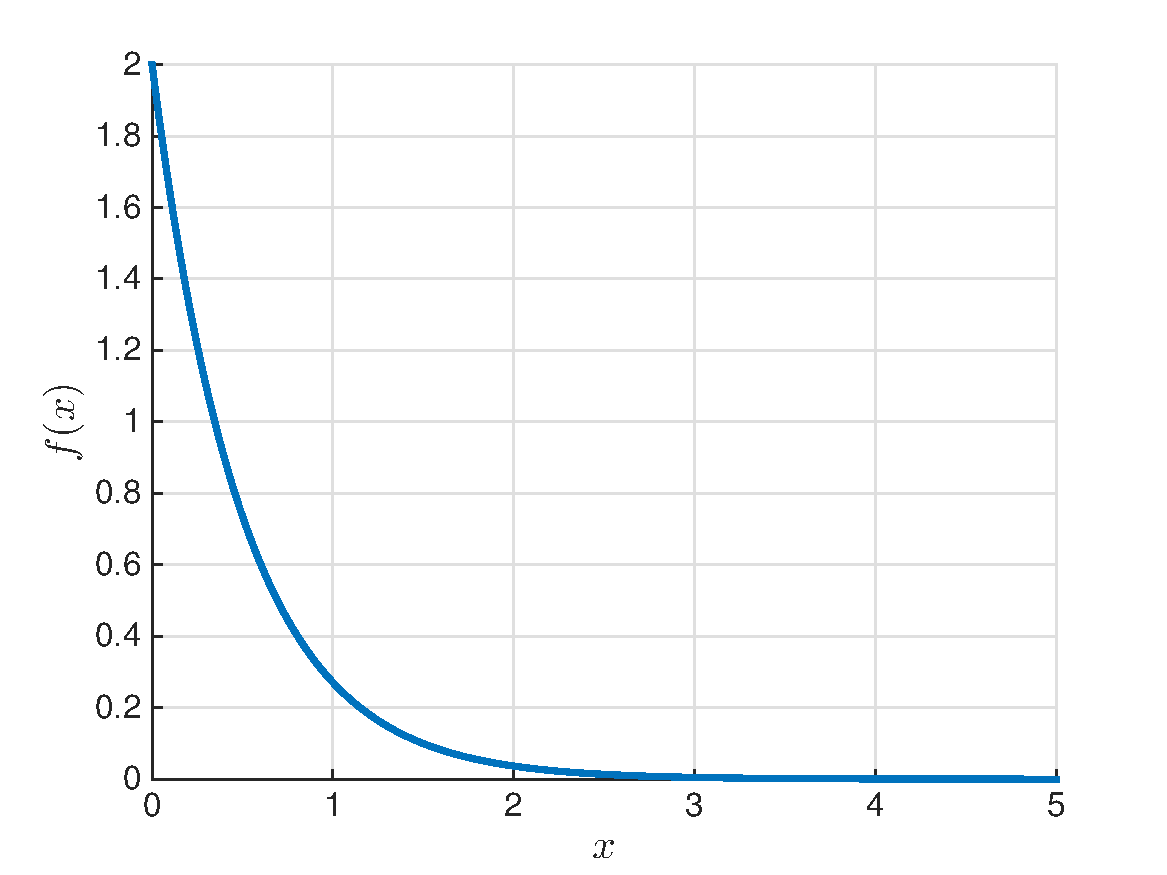
\includegraphics[scale=0.35]{exponential}
\caption{The density function for the exponential distribution with $\lambda = 2$.}
\label{fig:exponential}
\end{figure}

Let us now compute its expectation and variance.

\begin{theorem}
Let $X$ be an exponential random variable with parameter~$\lambda > 0$. Then
$$\Ex{X} = \frac{1}{\lambda} \qquad \text{ and } \qquad \Var{X} = \frac{1}{\lambda^2}.$$
\end{theorem}
\begin{proof}
We can calculate the expected value using integration by parts:
$$
   \Ex{X} = \int_{-\infty}^\infty xf(x) dx = \int_0^\infty \lambda xe^{-\lambda x}dx
             = \bigl[-xe^{-\lambda x}\bigr]_0^\infty + \int_0^\infty e^{-\lambda x} dx
             = 0 + \left[-\frac{e^{-\lambda x}}{\lambda}\right]_0^\infty = \frac{1}{\lambda}.  $$
To compute the variance, we first evaluate $\Ex{X^2}$, again using integration by parts:
$$ \Ex{X^2} = \int_{-\infty}^\infty x^2f(x) dx = \int_0^\infty \lambda x^2e^{-\lambda x}dx
             = \bigl[-x^2e^{-\lambda x}\bigr]_0^\infty + \int_0^\infty 2xe^{-\lambda x} dx
             = 0 + \frac{2}{\lambda}\Ex{X} = \frac{2}{\lambda^2}.  $$
The variance is therefore $$
   \Var{X} = \Ex{X^2} - \Ex{X}^2 = \frac{2}{\lambda^2} - \frac{1}{\lambda^2} = \frac{1}{\lambda^2},$$
as claimed.
\end{proof}


\subsubsection*{Exponential distribution is the continuous time analog of geometric distribution}

Like the geometric distribution, the exponential distribution has a single parameter~$\lambda$,
which characterizes the {\it rate\/} at which events happen.
Note that the exponential distribution satisfies, for any $t\ge 0$,
\begin{equation}\label{eq:exptail}
   \Pr[X> t] = \int_t^\infty \lambda e^{-\lambda x} dx = \bigl[-e^{-\lambda x}\bigr]_t^\infty
                  = e^{-\lambda t}.
\end{equation}
In other words, the probability that we have to wait more than time~$t$ for our event
to happen is $e^{-\lambda t}$, which is an exponential decay with rate~$\lambda$.

Now consider a discrete-time setting in which we perform one trial every $\delta$ seconds
(where $\delta$ is very small --- in fact, we will take $\delta\to 0$ to make time ``continuous"),
and where our success probability is $p=\lambda\delta$.
Making the success probability proportional to~$\delta$ makes sense, as it corresponds to
the natural assumption that there is a fixed {\it rate\/} of success {\it per unit time\/},
which we denote by $\lambda = p/\delta$.  In this discrete setting, the number of trials until we get a success
has the geometric distribution with parameter~$p$, so if we let the r.v.~$Y$ denote the
time (in seconds) until we get a success we have $$
   \Pr[Y> k\delta] = (1-p)^k = (1-\lambda\delta)^k \qquad\hbox{\rm for any $k\ge 0$}.  $$
Hence, for any $t>0$, we have
\begin{equation}\label{eq:geomtail}
   \Pr[Y> t] = \Pr[Y>({\textstyle\frac{t}{\delta}})\delta] = (1-\lambda\delta)^{t/\delta}
           \approx e^{-\lambda t},
\end{equation}
where this final approximation holds in the limit as $\delta\to 0$ with $\lambda$ and $t$
fixed.  (We are ignoring the detail of rounding $\frac{t}{\delta}$ to an integer since we
are taking an approximation anyway.)

Comparing the expression~\eqref{eq:geomtail} with~(\ref{eq:exptail}), we see that this distribution has the
same form as the exponential distribution with parameter~$\lambda$, where $\lambda$
(the success rate per unit time) plays an analogous role to~$p$ (the probability of success
on each trial) --- though note that $\lambda$ is not constrained to be $\le 1$.  Thus we may view
the exponential distribution as a continuous time analog of the geometric distribution.

\subsection*{Normal Distribution}

The last continuous distribution we will look at, and by far the
most prevalent in applications, is called the
{\it normal\/} or {\it Gaussian\/} distribution.  It has two parameters, $\mu$ and~$\sigma$,
which are the mean and standard deviation of the distribution, respectively.

\begin{definition}[Normal distribution]
For any $\mu \in \R$ and $\sigma> 0$, a continuous random variable~$X$
with pdf $$
   f(x) = \frac{1}{\sqrt{2\pi\sigma^2}} \,e^{-(x-\mu)^2/2\sigma^2}  $$
is called a \ul{normal random variable with parameters~$\mu$ and~$\sigma$}.
In the special case $\mu=0$ and $\sigma=1$, $X$ is said to have the
\ul{standard normal distribution}.
\end{definition}

Let's first check that this is a valid definition of a probability density function. Clearly $f(x) \ge 0$ from
the definition. For condition~(\ref{eq:total}):
\begin{equation}\label{eq:totalnormal}
   \int_{-\infty}^\infty f(x)dx = \frac{1}{\sqrt{2\pi\sigma^2}} \int_{-\infty}^\infty e^{-(x-\mu)^2/2\sigma^2} =1.
\end{equation}
The fact that this integral evaluates to~1 is a routine exercise in integral calculus, and is left
as an exercise (or feel free to look it up in any standard book on probability or on the internet).


A plot of the pdf~$f$ reveals a classical ``bell-shaped" curve, centered at (and symmetric
around) $x=\mu$, and with ``width" determined by~$\sigma$. 
Figure~\ref{fig:normal} shows the normal density for several different choices of $\mu$ and $\sigma$.

\begin{figure}[h!]
\centering
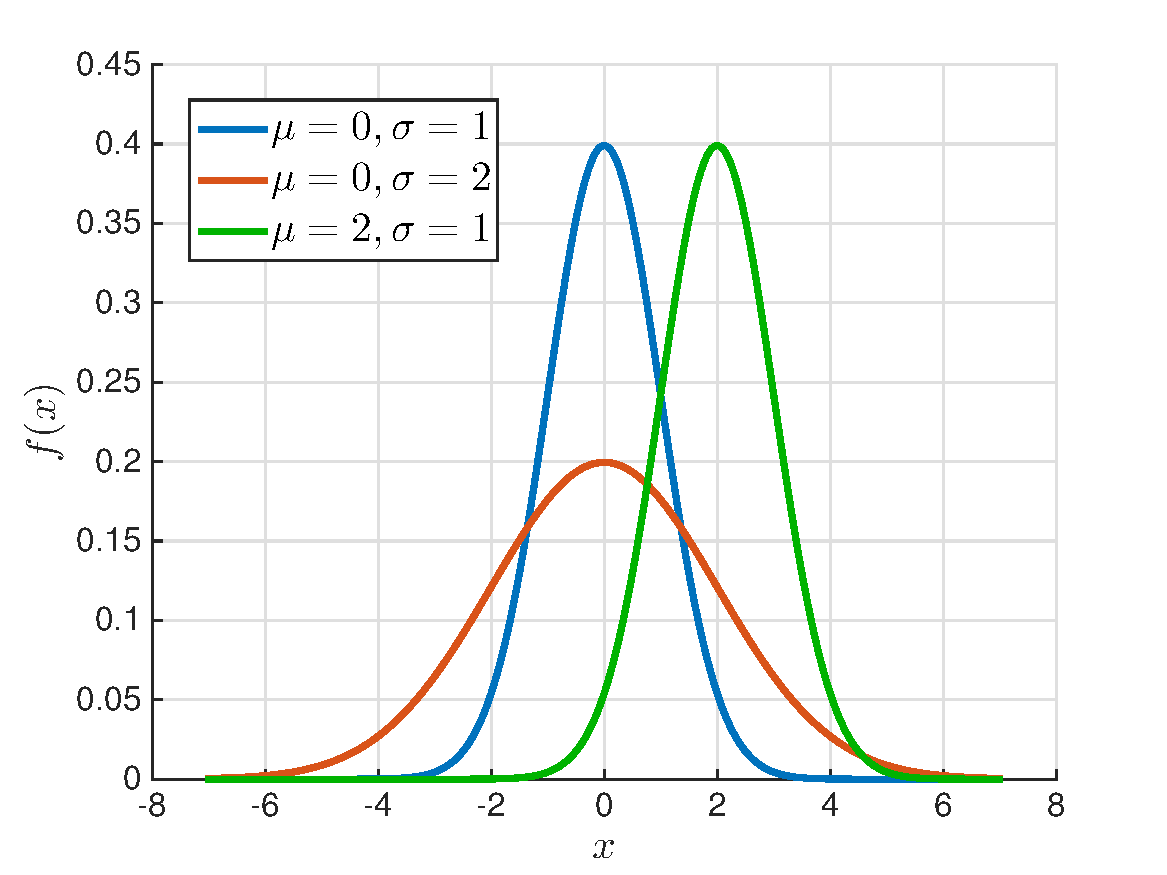
\includegraphics[scale=0.4]{normal}
\caption{The density function for the normal distribution with several different choices for $\mu$ and $\sigma$.}
\label{fig:normal}
\end{figure}

The figure above shows that the normal density with different values of $\mu$ and $\sigma$ are very similar to each other.
Indeed, the normal distribution has the following nice property with respect to shifting and rescaling.

\begin{lemma}\label{lem:normalshift}
If $X$ is a normal random variable with parameters $\mu$ and $\sigma$, then $Y = \frac{X - \mu}{\sigma}$
is a standard normal random variable. Equivalently, if $Y$ is a standard normal random variable, then
$X = \sigma Y + \mu$ has normal distribution with parameters $\mu$ and $\sigma$.
\end{lemma}
\begin{proof}
Given that $X$ has normal distribution with parameters $\mu$ and $\sigma$, we can calculate
the distribution of $Y=\frac{X-\mu}{\sigma}$ as:
$$   \Pr[a\le Y\le b] = \Pr[\sigma a+\mu \le X\le \sigma b+\mu] =
          \frac{1}{\sqrt{2\pi\sigma^2}}\int_{\sigma a+\mu}^{\sigma b+\mu} e^{-(x-\mu)^2/2\sigma^2} dx =
          \frac{1}{\sqrt{2\pi}}\int_{a}^{b} e^{-y^2/2} dy, $$
by a  simple change of variable $x = \sigma y + \mu$ in the integral.  Hence $Y$ is indeed standard normal.
Note that $Y$ is obtained from~$X$ just by shifting the origin to~$\mu$ and scaling by~$\sigma$.
\end{proof}


Let us now calculate the expectation and variance of a normal random variable.

\begin{theorem}
For a normal random variable $X$ with parameters $\mu$ and $\sigma$,
$$\Ex{X} = \mu \qquad \text { and } \qquad \Var{X} = \sigma^2.$$
\end{theorem}
\begin{proof}
Let's first consider the case when $X$ is standard normal, i.e., when $\mu = 0$ and $\sigma = 1$.
By definition, its expectation is $$
   \Ex{X} = \int_{-\infty}^\infty xf(x)dx = \frac{1}{\sqrt{2\pi}}\int_{-\infty}^\infty x e^{-x^2/2} dx =
           \frac{1}{\sqrt{2\pi}}\left(\int_{-\infty}^0 x e^{-x^2/2} dx +\int_{0}^\infty x e^{-x^2/2} dx \right) = 0.  $$
The last step follows from the fact that the function $e^{-x^2/2}$ is symmetrical about $x=0$,
so the two integrals are the same except for the sign.  For the variance, we have
\begin{eqnarray*}
   \Var{X} = \Ex{X^2} - \Ex{X}^2 &=& \frac{1}{\sqrt{2\pi}}\int_{-\infty}^\infty x^2 e^{-x^2/2} dx \\
                &=& \frac{1}{\sqrt{2\pi}}\bigl[-xe^{-x^2/2}\bigr]_{-\infty}^\infty
                        + \frac{1}{\sqrt{2\pi}}\int_{-\infty}^\infty e^{-x^2/2} dx \\
                &=& \frac{1}{\sqrt{2\pi}} \int_{-\infty}^\infty e^{-x^2/2} dx = 1.
\end{eqnarray*}
In the first line here we used the fact that $\Ex{X}=0$; in the second line we used integration
by parts; and in the last line we used~(\ref{eq:totalnormal}) in the special case $\mu=0$, $\sigma=1$.
So the standard normal distribution has expectation $\Ex{X}=0=\mu$ and variance
$\Var{X}=1=\sigma^2$.

Now consider the general case when $X$ has normal distribution with general parameters
$\mu$ and $\sigma$. By Lemma~\ref{lem:normalshift}, we know that $Y = \frac{X-\mu}{\sigma}$
is a standard normal random variable, so $\Ex{Y} = 0$ and $\Var{Y} = 1$, as we have just established above.
Therefore, we can read off the expectation and variance of~$X$ from those of~$Y$.  For the
expectation, using linearity, we have $$
   0 = \Ex{Y} = \hbox{\rm E}\left(\frac{X-\mu}{\sigma}\right) = \frac{\Ex{X}-\mu}{\sigma},  $$
and hence $\Ex{X} = \mu$.   For the variance we have $$
   1 = \Var{Y} = \hbox{\rm Var}\left(\frac{X-\mu}{\sigma}\right) = \frac{\Var{X}}{\sigma^2},  $$
and hence $\Var{X}=\sigma^2$.
\end{proof}

The bottom line, then, is that the normal distribution has expectation~$\mu$ and
variance~$\sigma^2$. This explains the notation for the parameters~$\mu$ and $\sigma$.

The fact that the variance is~$\sigma^2$ (so that the standard deviation is~$\sigma$)
explains our earlier comment that $\sigma$ determines the ``width'' of the normal
distribution.  Namely, by Chebyshev's inequality, a constant fraction of the distribution
lies within distance (say) $2\sigma$ of the expectation~$\mu$.

{\bf Note:} The above analysis shows that, by means of a simple origin shift and scaling,
we can relate any normal distribution to the standard normal.  This means that, when doing
computations with normal distributions, it's enough to do them for the standard normal.
For this reason, books and online sources of mathematical formulas usually contain tables
describing the density of the standard normal.  From this, one can read off the corresponding
information for any normal r.v.~$X$ with parameters $\mu,\sigma^2$, from the formula $$
   \Pr[X\le a] = \Pr[Y\le {\textstyle\frac{a-\mu}{\sigma}}],  $$
where $Y$ is standard normal.

The normal distribution is ubiquitous throughout the sciences and
the social sciences, because it is the standard model for any
aggregate data that results from a large number of independent
observations of the same random variable (such as the heights of
females in the US population, or the observational error in a
physical experiment). Such data, as is well known, tends to cluster
around its mean in a ``bell-shaped" curve, with the correspondence
becoming more accurate as the number of observations increases. A
theoretical explanation of this phenomenon is the Central Limit
Theorem, which we next discuss.


\subsubsection*{Sum of Independent Normal Random Variables}

An important property of the normal distribution is that the sum of {\em independent}
normal random variables is also normally distributed. We begin with the simple case when
$X$ and $Y$ are independent standard normal random variables. In this case the result follows
because the joint distribution of $X$ and $Y$ is rotationally symmetric. The general case follows
from the translation and scaling property of normal distribution in Lemma~\ref{lem:normalshift}.


\begin{theorem}\label{thm:normalsum}
Let $X$ and $Y$ be independent standard normal random variables, and $a,b \in \mathbb{R}$ be constants. Then
$Z = aX + bY$ is also a normal random variable with parameters $\mu = 0$ and $\sigma^2 = a^2 + b^2$.
\end{theorem}
\begin{proof}\footnote{The following proof and figures are adapted from~{\em ``Why Is the Sum of Independent Normal Random Variables Normal?''} by B.~Eisenberg and R.~Sullivan, Mathematics Magazine, Vol.~81, No.~5.}
Since $X$ and $Y$ are independent, by Theorem~\ref{Thm:JointDensity} we know that the joint density of $(X,Y)$ is
$$f(x,y) = f(x) \cdot f(y) = \frac{1}{2\pi} e^{-(x^2+y^2)/2}.$$
The key observation is that $f(x,y)$ is rotationally symmetric around the origin, i.e., $f(x,y)$ only depends on the value $x^2 + y^2$,
which is the distance of the point $(x,y)$ from the origin $(0,0)$; see Figure~\ref{fig:jointnormal}.

\begin{figure}[h!]
\centering
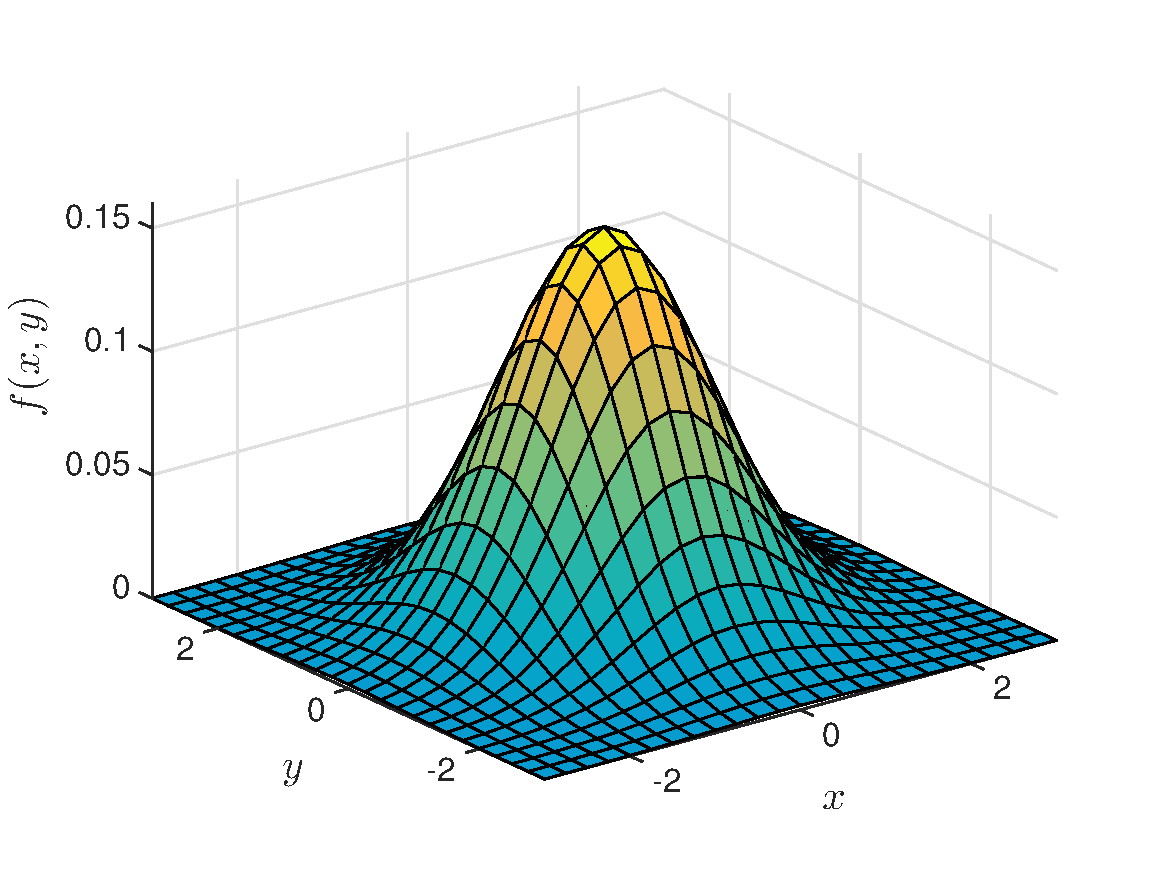
\includegraphics[scale=0.4]{jointnormal}
\caption{The joint density function $f(x,y) = \frac{1}{2\pi} e^{-(x^2+y^2)/2}$ is rotationally symmetric.}
\label{fig:jointnormal}
\end{figure}

 Thus, $f(T(x,y)) = f(x,y)$ where $T$ is any rotation of the plane
$\mathbb{R}^2$ about the origin. It follows that for any set $A \subseteq \mathbb{R}^2$,
\begin{equation}\label{Eq:NormalRotation}
\Pr[(X,Y) \in A] = \Pr[(X,Y) \in T(A)]
\end{equation}
where $T$ is a rotation of $\mathbb{R}^2$. Now given any $t \in \mathbb{R}$, we have
$$\Pr[Z \le t] ~=~ \Pr[aX + bY \le t] ~=~ \Pr[(X,Y) \in A]$$
where $A$ is the half plane $\{(x,y) \mid ax + by \le t\}$. The boundary line $ax+by = t$ lies at a distance
$d = \frac{t}{\sqrt{a^2 + b^2}}$ from the origin. Therefore, as illustrated in Figure~\ref{fig:normalrotation}, the set $A$ can be rotated into the set
$$T(A) = \big\{(x,y) \: \big| \; x \le \frac{t}{\sqrt{a^2+b^2}} \big\}.$$

\begin{figure}[h!]
\centering
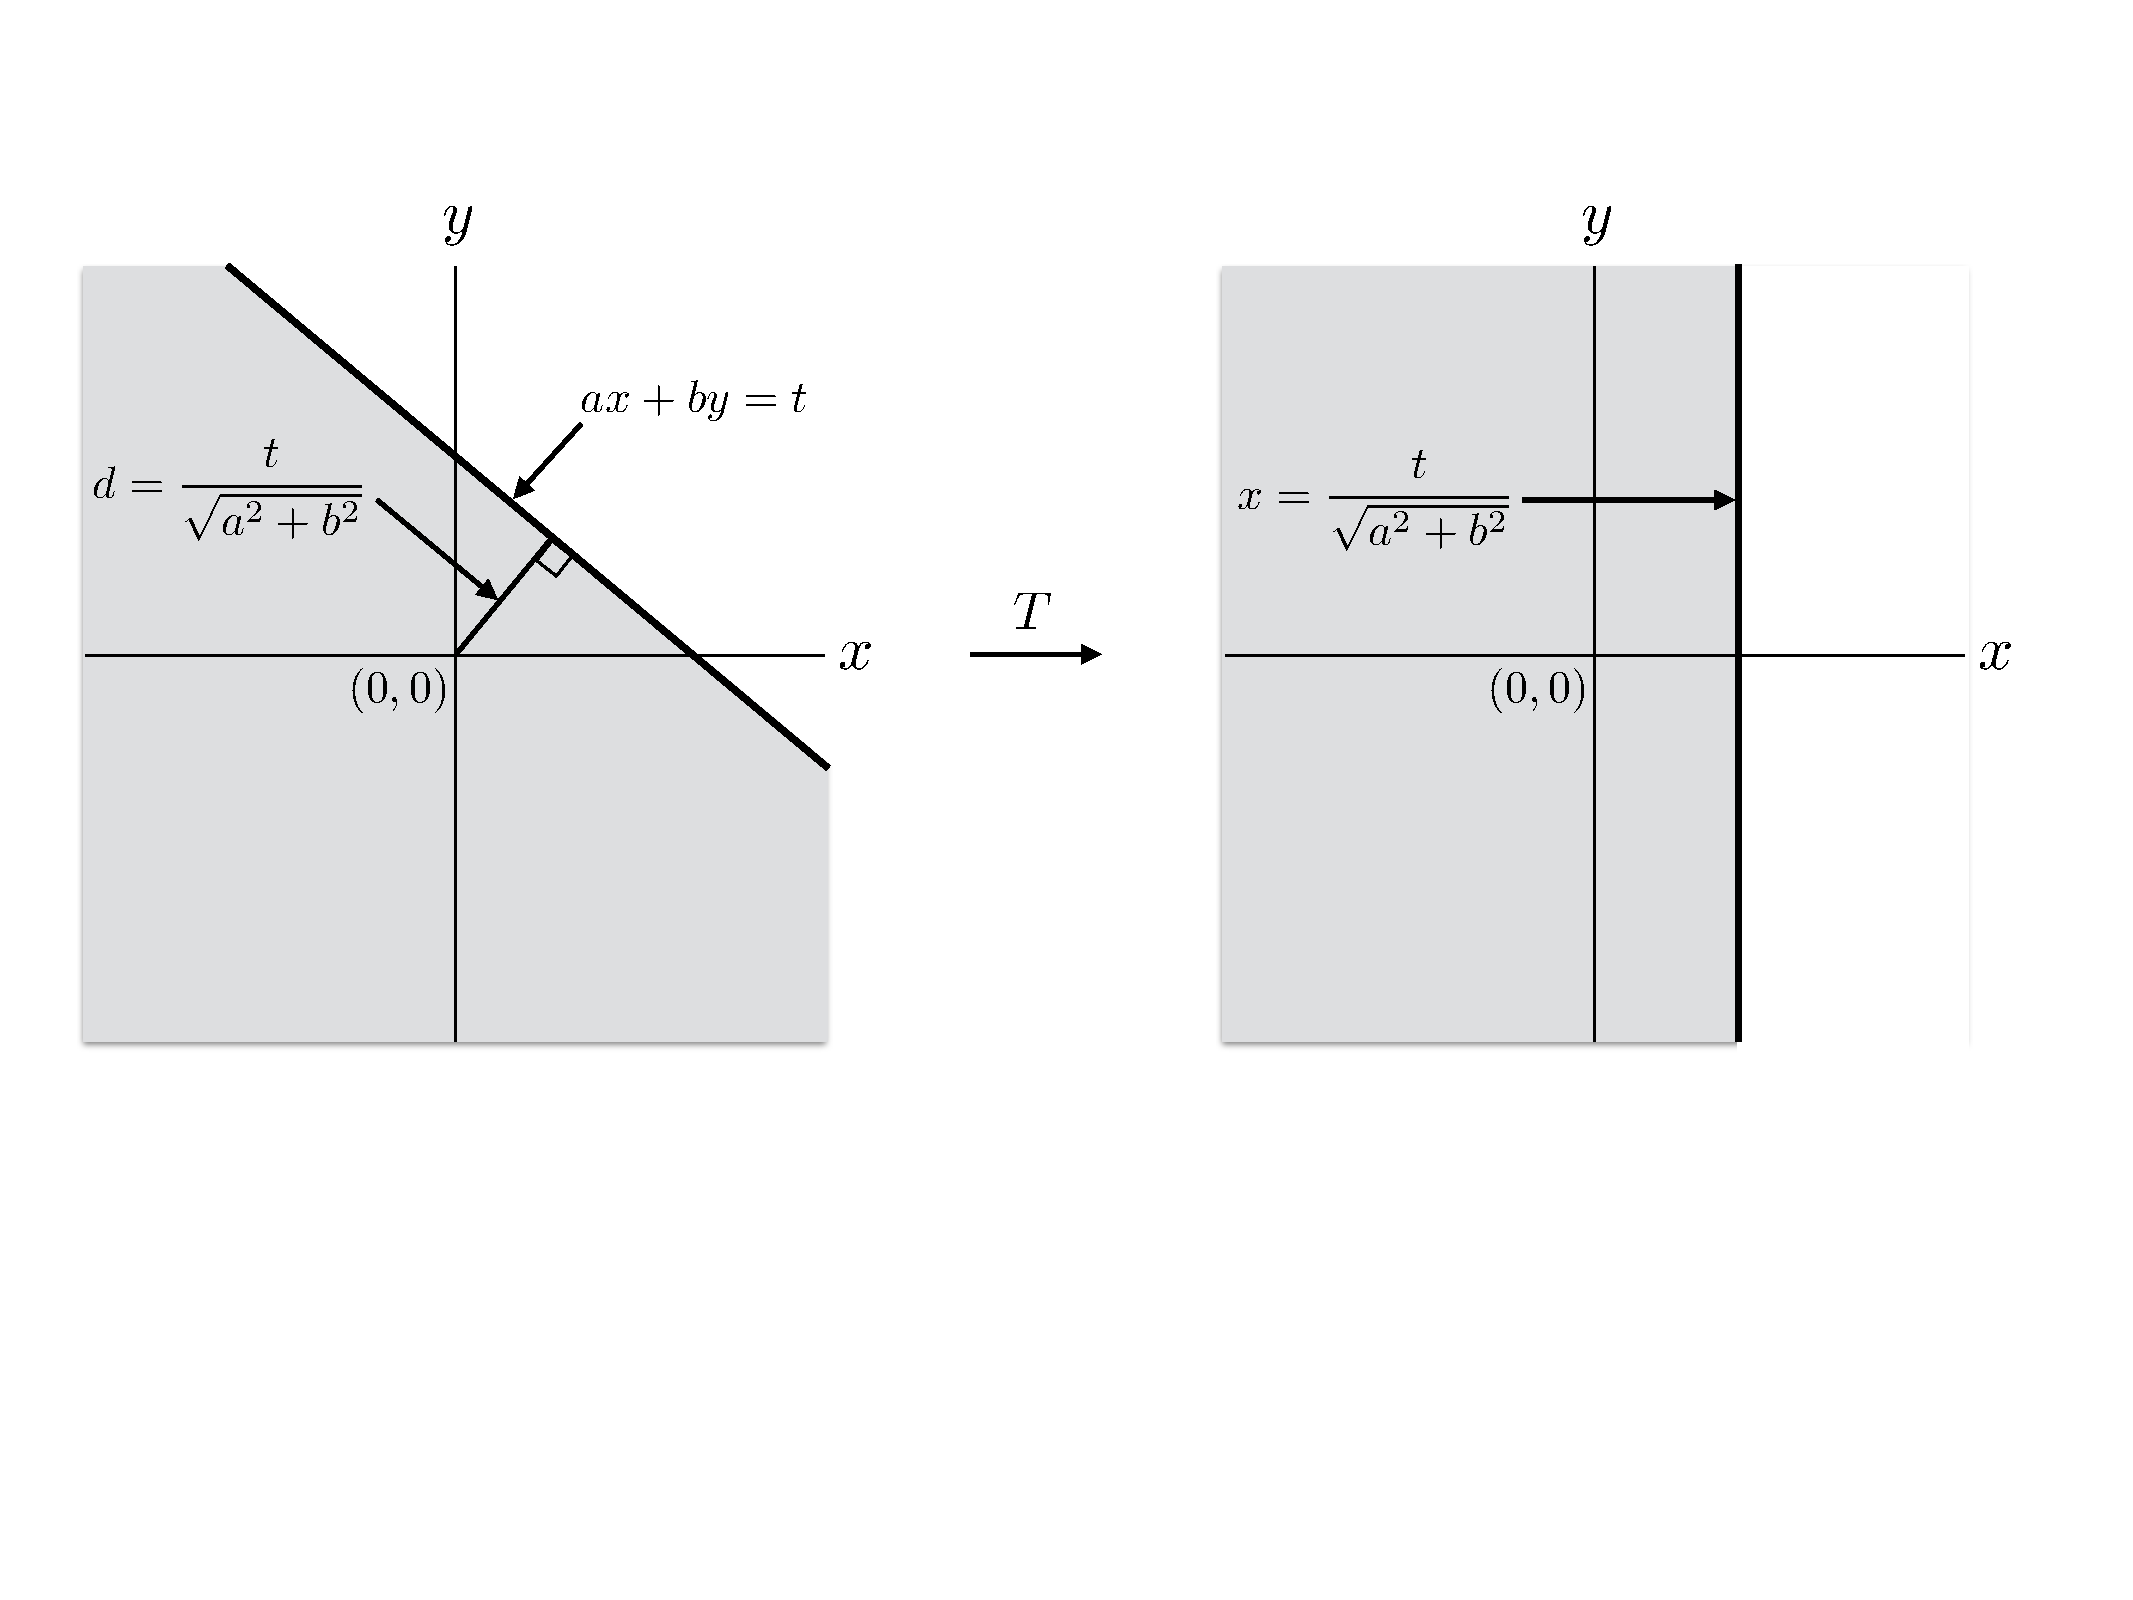
\includegraphics[scale=0.35]{normalrotation}
\caption{The half plane $ax+by \le t$ is rotated into the half plane $x \le \frac{t}{\sqrt{a^2+b^2}}$.}
\label{fig:normalrotation}
\end{figure}

By~\eqref{Eq:NormalRotation}, this rotation does not change the probability:
$$\Pr[Z \le t] ~=~ \Pr[(X,Y) \in A] ~=~ \Pr[(X,Y) \in T(A)] ~=~ \Pr\Big[X \le \frac{t}{\sqrt{a^2+b^2}} \Big] ~=~ \Pr[\sqrt{a^2+b^2} \, X \le t].$$
Since the equation above holds for all $t \in \R$, we conclude that $Z $ has the same distribution as $\sqrt{a^2+b^2} \, X$. Since $X$ has standard normal distribution, we know by Lemma~\ref{lem:normalshift} that $\sqrt{a^2 + b^2} \, X$ has normal distribution with mean $0$ and variance $a^2+b^2$. Hence we conclude that $Z = aX + bY$ also has normal distribution with mean $0$ and variance $a^2+b^2$.
\end{proof}


The general case now follows easily from Lemma~\ref{lem:normalshift} and Theorem~\ref{thm:normalsum}.

\begin{corollary}
Let $X$ and $Y$ be independent normal random variables with parameters $(\mu_X, \sigma^2_X)$ and $(\mu_Y, \sigma^2_Y)$, respectively. Then for any constants $a,b \in \R$, the random variable $Z = aX + bY$ is also normally distributed with mean $\mu = a\mu_X + b \mu_Y$ and variance $\sigma^2 = a^2 \sigma_X^2 + b^2 \sigma_Y^2$.
\end{corollary}
\begin{proof}
By Lemma~\ref{lem:normalshift}, $Z_1 = (X - \mu_X) / \sigma_X$ and $Z_2 = (Y - \mu_Y) / \sigma_Y$ are independent standard normal random variables. We can write:
\begin{align*}
Z ~&=~ aX + bY
~=~ a(\mu_X + \sigma_X Z_1) + b(\mu_Y + \sigma_Y Z_2)
~=~ (a\mu_X + b\mu_Y) + (a\sigma_X Z_1 + b\sigma_Y Z_2).
\end{align*}
By Theorem~\ref{thm:normalsum}, $Z' = a\sigma_X Z_1 + b\sigma_Y Z_2$ is normally distributed with mean $0$ and variance
$\sigma^2 = a^2 \sigma_X^2 + b^2 \sigma_Y^2$. Since $\mu = a\mu_X + b\mu_Y$ is a constant, by Lemma~\ref{lem:normalshift} we conclude that $Z = \mu + Z'$ is a normal random variable with mean $\mu$ and variance $\sigma^2$, as desired.
\end{proof}




\section*{The Central Limit Theorem}

Recall from Note~18 the Law of Large Numbers for i.i.d.\
random variables $X_i$'s: it says that the probability of {\it any\/}
deviation~$\alpha$ of the sample average $A_n :=
\frac{1}{n}{\sum_{i=1}^n X_i}$ from the mean, however small, tends
to zero as the number of observations~$n$ in our average tends to
infinity. Thus by taking $n$ large enough, we can make the
probability of any given deviation as small as we like.

Actually we can say something much stronger than the Law of Large
Numbers: namely, the distribution of the sample average~$A_n$, for
large enough~$n$, looks like a {\it normal distribution\/} with
mean~$\mu$ and variance $\frac{\sigma^2}{n}$.  (Of course, we
already know that these are the mean and variance of~$A_n$; the
point is that the distribution becomes normal!)  The fact that the
standard deviation decreases with~$n$ (specifically, as
$\frac{\sigma}{\sqrt{n}}$) means that the distribution approaches a
sharp spike at~$\mu$.

Recall from the last section that the density of the normal distribution
is a symmetrical bell-shaped curve centered around the mean~$\mu$.
Its height and width are determined by the standard
deviation~$\sigma$ as follows: the height at the mean $x = \mu$ is $\frac{1}{\sqrt{2\pi \sigma^2}} \approx \frac{0.4}{\sigma}$; 
50\% of the mass is contained in the interval of
width $0.67\sigma$ either side of the mean, and 99.7\% in the
interval of width $3\sigma$ either side of the mean. (Note that, to
get the correct scale, deviations are on the order of~$\sigma$
rather than~$\sigma^2$.)

To state the Central Limit Theorem precisely (so that the limiting
distribution is a constant rather than something that depends
on~$n$), we shift the mean of~$A_n$ to~0 and scale it so that its
variance is~1, i.e., we replace~$A_n$ by $$
   A'_n = \frac{(A_n-\mu)\sqrt{n}}{\sigma} = \frac{\sum_{i=1}^n X_i -n\mu}{\sigma\sqrt{n}}.  $$
The Central Limit Theorem then says that the distribution of~$A'_n$
converges to the {\it standard normal\/} distribution.

\begin{theorem}[{\bf Central Limit Theorem}]
Let $X_1,X_2,\ldots,X_n$ be i.i.d.\ random variables with common
expectation $\mu=\Ex{X_i}$ and variance $\sigma^2=\Var{X_i}$ (both
assumed to be $<\infty$).  Define $A'_n = \frac{\sum_{i=1}^n X_i
-n\mu}{\sigma\sqrt{n}}$. Then as $n\to\infty$, the distribution of
$A'_n$ approaches the standard normal distribution in the sense
that, for any real~$\alpha$, $$
   \Pr[A'_n \le \alpha] \to \frac{1}{\sqrt{2\pi}}\int_{-\infty}^\alpha e^{-x^2/2}dx\quad\hbox{\rm as $n\to\infty$}.  $$
\end{theorem}

The Central Limit Theorem is a very striking fact.  What it says is
the following:  If we take an average of $n$ observations of
 any arbitrary r.v.~$X$, then the distribution of that average will
be a bell-shaped curve centered at $\mu=\Ex{X}$.  Thus all trace of
the distribution of~$X$ disappears as $n$ gets large: all
distributions, no matter how complex,\footnote{We do need to assume
that the mean and variance of~$X$ are finite.} look like the normal
distribution when they are averaged.  The only effect of the
original distribution is through the variance~$\sigma^2$, which
determines the width of the curve for a given value of~$n$, and
hence the rate at which the curve shrinks to a spike.


\section*{Optional: Buffon's Needle}

Here is a simple yet interesting application of continuous random variables to the analysis
of a classical procedure for estimating the value of~$\pi$ known as {\it Buffon's
needle}, after its 18th century inventor Georges-Louis Leclerc, Comte de Buffon.

Here we are given a needle of length~$\ell$, and a board ruled with
horizontal lines at distance~$\ell$ apart.  The experiment consists
of throwing the needle randomly onto the board and observing whether
or not it crosses one of the lines. We shall see below that
(assuming a perfectly random throw) the probability of this event is
exactly~$2/\pi$.  This means that, if we perform the experiment many
times and record the {\it proportion\/} of throws on which the
needle crosses a line, then the Law of Large Numbers
tells us that we will get a good estimate of the quantity~$2/\pi$,
and therefore also of~$\pi$; and we can use Chebyshev's inequality
as in the other estimation problems we considered in that same Note 
to determine how many throws we need in order 
to achieve specified accuracy and confidence.

To analyze the experiment, let's consider what random variables are in play.  Note that the
position where the needle lands is completely specified by two
random variables: the vertical distance~$Y$ between the midpoint of
the needle and the closest horizontal line, and the angle~$\Theta$
between the needle and the vertical.  The r.v.~$Y$ ranges between~0
and~$\ell/2$, while $\Theta$ ranges between $-\pi/2$  and~$\pi/2$.
Since we assume a perfectly random throw, we may assume that their
{\it joint distribution\/} has density $f(y,\theta)$ that is uniform
over the rectangle $[0,\ell/2]\times[-\pi/2,\pi/2]$. Since this
rectangle has area $\frac{\pi\ell}{2}$, the density should be
\begin{equation}\label{eq:ytheta}
   f(y,\theta) = \begin{cases}
       2/\pi\ell & \hbox{\rm for $(y,\theta)\in [0,\ell/2]\times[-\pi/2,\pi/2]$;}\cr
       0 & \hbox{\rm otherwise}.\cr
   \end{cases}
\end{equation}
Equivalently, $Y$ and $\Theta$ are independent random variables, each uniformly distributed in their respective range.
As a sanity check, let's verify that the integral of this density over all possible
values is indeed~1:  $$
   \int_{-\infty}^\infty \int_{-\infty}^\infty f(y,\theta) dy d\theta
        = \int_{-\pi/2}^{\pi/2}\int_0^{\ell/2} \frac{2}{\pi\ell} dyd\theta
        = \int_{-\pi/2}^{\pi/2} \left[\frac{2y}{\pi\ell}\right]_0^{\ell/2} d\theta
        = \int_{-\pi/2}^{\pi/2} \frac{1}{\pi} d\theta
        = \left[\frac{\theta}{\pi}\right]_{-\pi/2}^{\pi/2}
        = 1.  $$
This is an analog of equation~(\ref{eq:total}) for our joint distribution; rather than
the area under the curve $f(x)$, we are now computing the area under the
``surface" $f(y,\theta)$. 

Now let $E$ denote the event that the needle crosses a line.  How can we
express this event in terms of the values of $Y$ and~$\Theta$?  Well, by
elementary geometry the vertical distance of the endpoint of the needle from
its midpoint is $\frac{\ell}{2}\cos\Theta$, so the needle will cross
the line if and only if $Y\le \frac{\ell}{2}\cos\Theta$.  Therefore we have $$
   \Pr[E] = \Pr[Y \le {\textstyle\frac{\ell}{2}}\cos\Theta] =
\int_{-\pi/2}^{\pi/2}\int_0^{(\ell/2)\cos\theta}
f(y,\theta)dyd\theta.
$$

Substituting the density $f(y,\theta)$ from equation~(\ref{eq:ytheta}) and performing
the integration we get
\begin{equation*}
    \Pr[E] = \int_{-\pi/2}^{\pi/2}\int_0^{(\ell/2)\cos\theta} \frac{2}{\pi\ell} dyd\theta
               = \int_{-\pi/2}^{\pi/2} \left[\frac{2y}{\pi\ell}\right]_0^{(\ell/2)\cos\theta}d\theta
               = \frac{1}{\pi}\int_{-\pi/2}^{\pi/2} \cos\theta d\theta
               = \frac{1}{\pi}\left[\sin\theta\right]_{-\pi/2}^{\pi/2}
               = \frac{2}{\pi}.
\end{equation*}

This is exactly what we claimed at the beginning of the section!

\subsection*{Buffon's Needle: A Slick Approach}

\begin{figure}[h]
\begin{center}
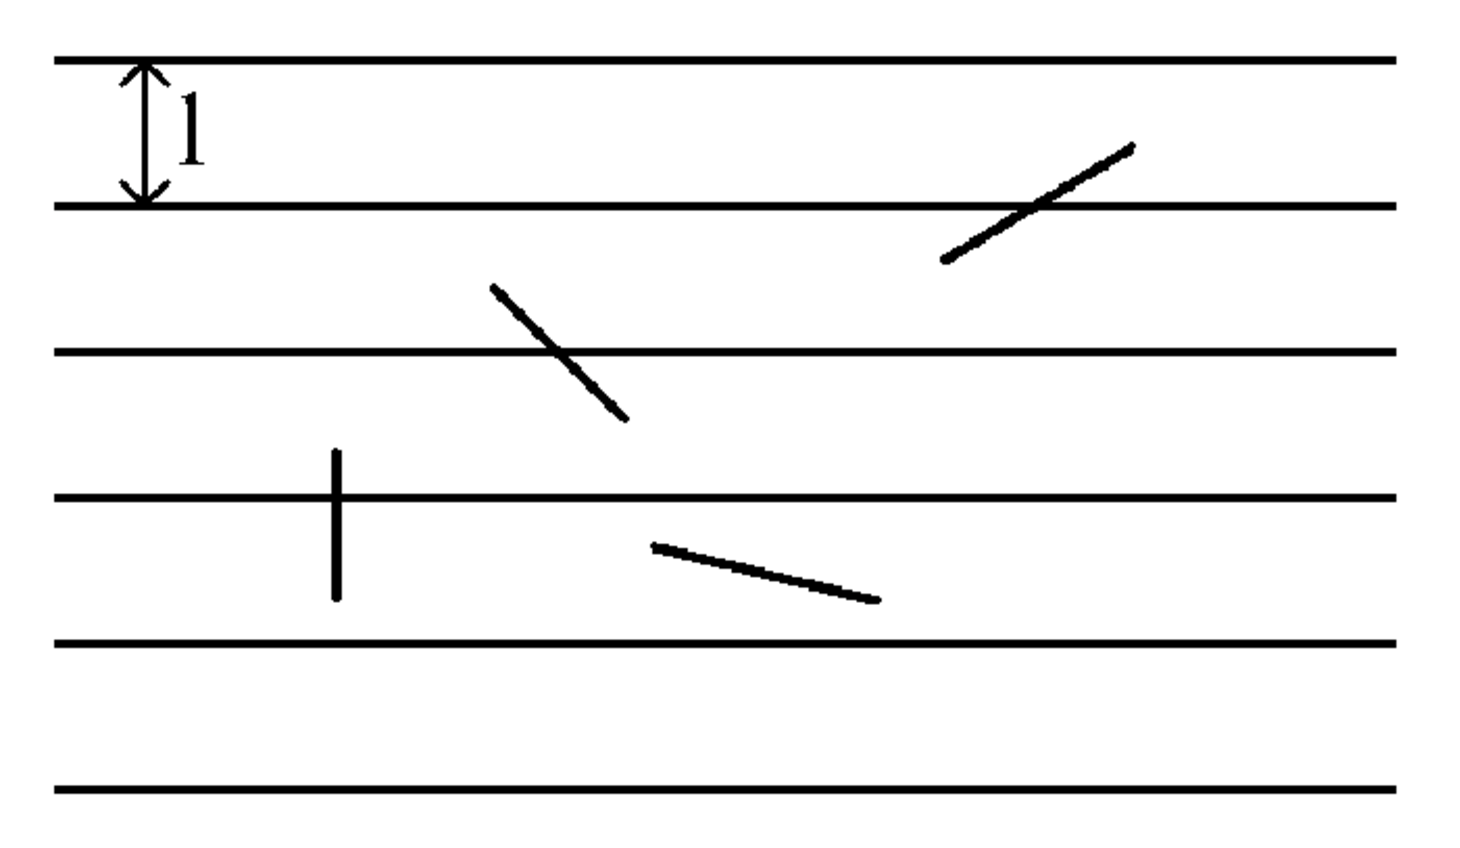
\includegraphics[scale=0.4]{needle.pdf}
\end{center}
\caption{Buffon's Needle.}
\label{fig:needle}
\end{figure}



Recall that we toss a unit length needle on (an infinite) board ruled with horizontal
lines spaced at unit length apart.  We wish to calculate
the chance that the needle intersects a horizontal line.  That is, let $I$ be the event that
the needle intersects a line.  We will show that $\Pr[I] = \frac{2}{\pi}$.  Let
$X$ be a random variable defined to be the number of intersections of such a needle:
$$X = \left\{ \begin{array}{cc}
1&\mbox{ if the needle intersects a line }\\
0&\mbox{ otherwise. }
\end{array}\right.$$

Since $X$ is an indicator random variable,  $\Ex{X} = \Pr[I] $
(here we are assuming the case in which the needle lies perfectly on two lines cannot happen, since
the probability of this particular event is $0$).
Now, imagine that we were tossing a needle of two unit length, and we let $Z$ be the random
variable representing the number of times such a needle intersects horizontal lines on the plane.
We can ``split" the needle into two parts of unit length and get $Z = X_1 + X_2$, where $X_i$
is $1$ if segment $i$ of the needle intersects and $0$ otherwise.  Thus, $\Ex{Z} = \Ex{X_1 + X_2}
= \Ex{X_1} + \Ex{X_2} = 2\Ex{X}$, since each segment is of unit length.  A similar argument holds
if we split a unit length needle into $m$ equal segments, so that $X = X_1 + \cdots + X_m$, where $X_i$
is $1$ if segment $i$ (which has length $\frac{1}{m}$) intersects a line and $0$ otherwise.  We have
that $\Ex{X} = \Ex{X_1 + \cdots + X_m} = \Ex{X_1} + \cdots + \Ex{X_m}$.  But each of the $\Ex{X_i}$'s are
equal, so we get $\Ex{X} = m\Ex{X_i} \rightarrow \Ex{X_i} = ($length of segment $i$)$\cdot \Ex{X}$.
Thus, if we drop a needle of length $l$, and we let $Y$ be the number of intersections, then
$\Ex{Y} = l \cdot \Ex{X}$.  Even if we have a needle which is arbitrarily short, say length $\epsilon$, we
still have $\Ex{Y} = \epsilon \cdot \Ex{X}$.  

\begin{figure}[h]
\begin{center}
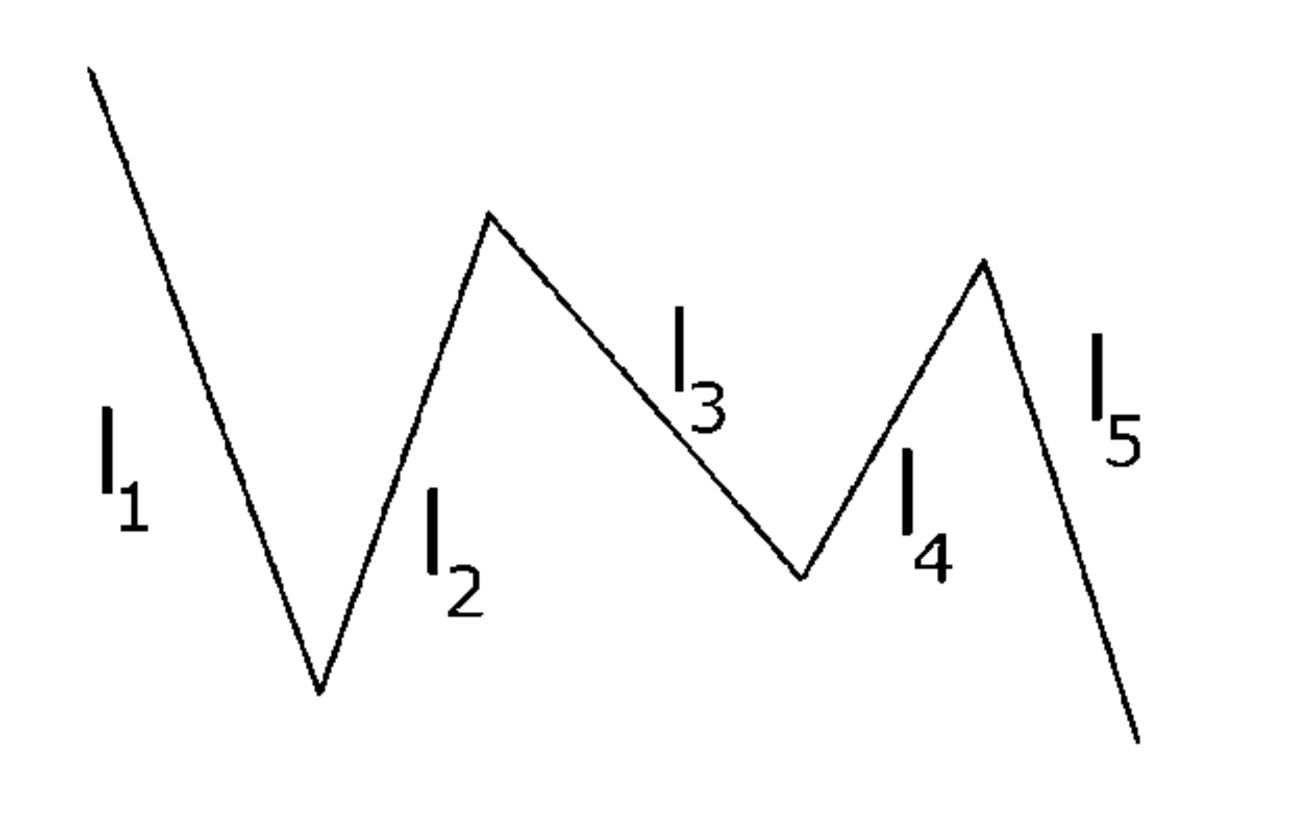
\includegraphics[scale=0.4]{noodle.pdf}
\end{center}
\caption{"Noodle" consisting of $5$ needles.}
\label{fig:noodle}
\end{figure}


Now, consider a ``noodle" comprised of
two needles of arbitrary lengths $l_1$ and $l_2$ (with corresponding random variables $X_1$ and $X_2$),
where the needles are connected by a rotating joint, we can conclude by linearity of expectation that
$\Ex{X_1 + X_2} = \Ex{X_1} + \Ex{X_2}$.  In general, we can have a noodle comprised of $n$ needles
of arbitrary length:
where $\Ex{X_1 + \cdots + X_n} = \Ex{X_1} + \cdots + \Ex{X_n} = l_1\Ex{X} + \cdots + l_n\Ex{X}$.  Factoring
$\Ex{X}$ out, we get that the expected number of intersections of a noodle is $($length of noodle$) \cdot \Ex{X}$.
In particular, since we are allowed to string together needles at connected rotating joints and since each needle
can be arbitrarily short, we are free to pick any shape, but which one?  

\begin{figure}[h]
\begin{center}
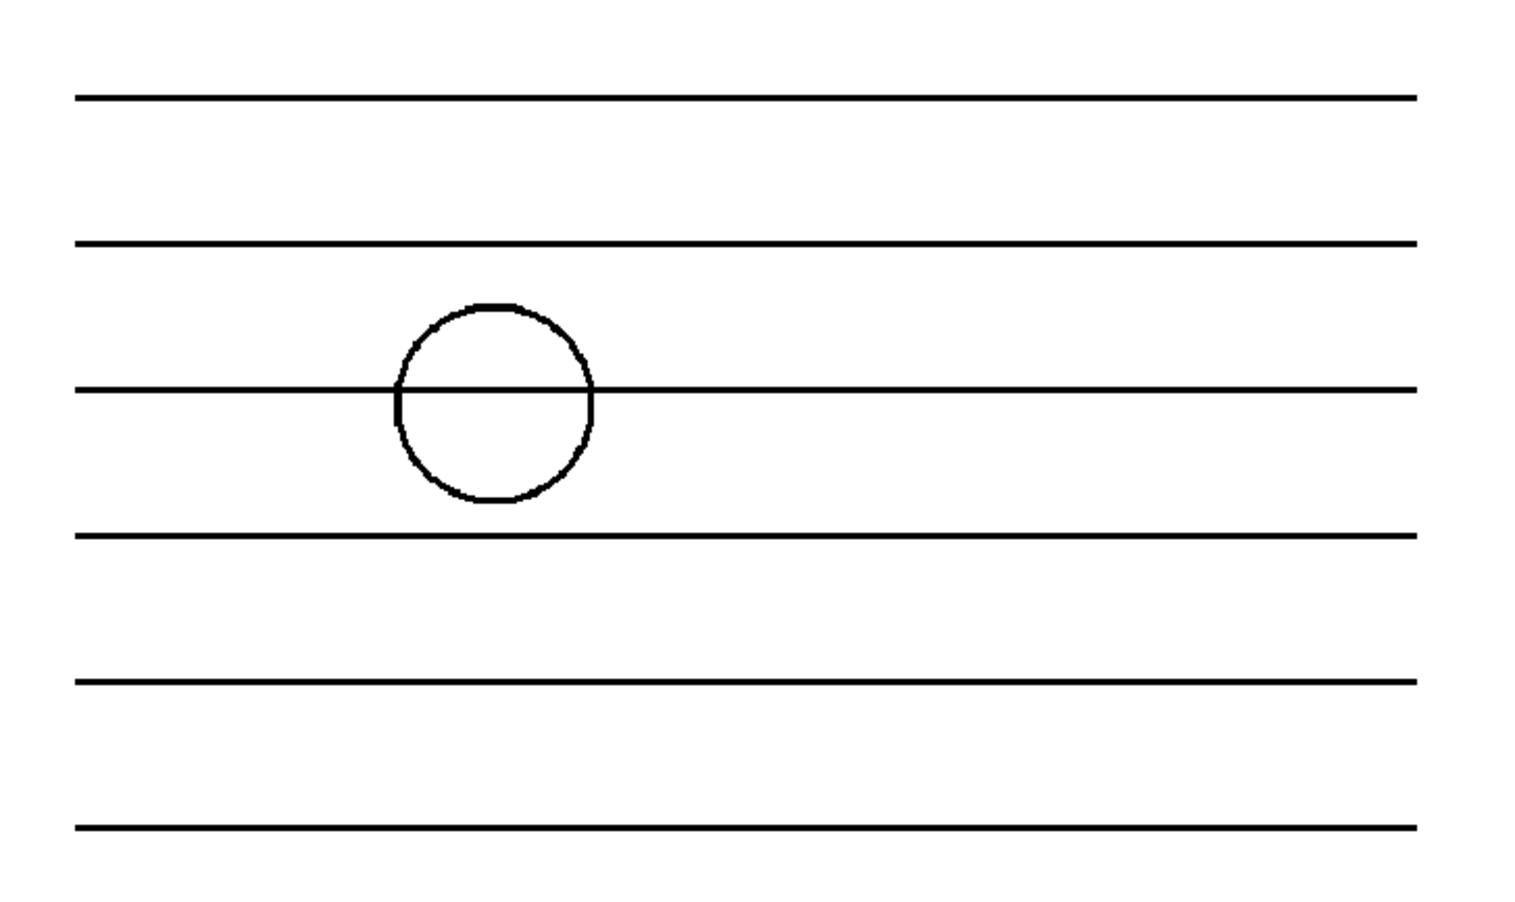
\includegraphics[scale=0.4]{circle.pdf}
\end{center}
\caption{A circle always has two intersections.}
\label{fig:circle}
\end{figure}

Consider a circle with a unit
length diameter (and therefore circumference $\pi$).  Such a shape must always intersect twice:
which implies $\Ex{$number of circle intersections$} = \pi \cdot \Ex{X} = 2$, and
thus $\Ex{X} = \frac{2}{\pi} = \Pr[I]$.


\end{document}
